\section{Maquina de Turing}
\subsection{ Descripci\'on del programa}
\justify
El siguiente programa es la Maquina de Turing, esta evalua si una cadena cuenta con la condici\'on de ser $0^n 1^n $ con n $>=$ 1.\\
Se mostrara en un archivo de texto la forma en la que esta se evalua y como van cambiando entre sus estados, asimismo se mostrara en otro archivo las cadenas que fueron aceptadas por la maquina.\\
La maquina de Turing es la siguiente.\\

\begin{figure}[H]
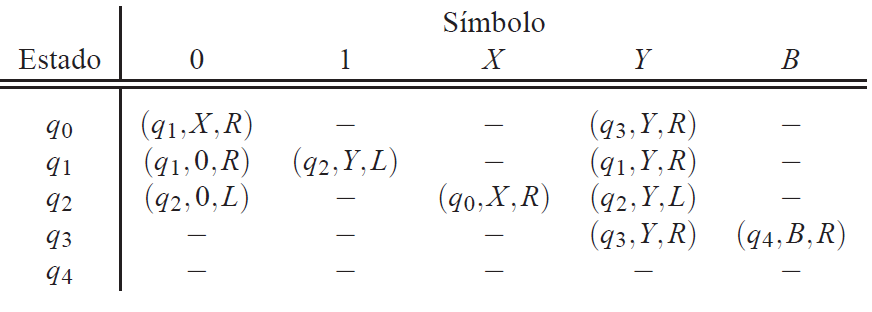
\includegraphics[width=\textwidth, height=7cm]{MT.png}
\label{fig:MT}
\caption{Maquina de Turing que acepta $0^n 1^n$ con n $>=1$}
\end{figure}

\subsection{C\'odigo}
El c\'digo utilizado para la resoluci\'on del problema se muestra a continuaci\'on:\\

C\'odigo:MaquinaTuring.py

\lstset{language=Python, breaklines=true, basicstyle=\footnotesize}
\begin{lstlisting}[frame=single]
	def maquinaTuring(cadena,archivo):
    estado=[0,"",0]
    cadena=list(cadena)
    index=0
    while True:
        for e in cadena:
            archivo.write(e)
        archivo.write("\n")
        for i in range(index):
            archivo.write(" ")
        archivo.write("|")
        archivo.write("\n")
        for i in range(index):
            archivo.write(" ")
        archivo.write("q"+str(estado[0])+"\n")
        try:
            if(index<0):
                raise Exception
            elif(estado[0]==0):
                estado[0]=estadoCero(cadena,index,estado)
                index=estado[2]
            elif(estado[0]==1):

                estado[0]=estadoUno(cadena,index,estado)
                index=estado[2]

            elif(estado[0]==2):
                estado[0]=estadoDos(cadena,index,estado)
                index=estado[2]
            elif(estado[0]==3):
                estado[0]=estadoTres(cadena,index,estado)
                index=estado[2]
            elif(estado[0]==4 or estado[0]==-1):
                break
            else:
                break
        except Exception as ex:
            if(estado[0]==3):
                estado[0]=4
            else:
                break
    return estado[0]
def estadoCero(cadena,index,estado):
    if(cadena[index]=='0'):
        cadena[index]='X'
        estado[1]="X"
        estado[2]=estado[2]+1
        return 1
    elif(cadena[index]=='Y'):
        cadena[index]='Y'
        estado[1]="Y"
        estado[2]=estado[2]+1
        return 3
    else:
        return -1

def estadoUno(cadena,index,estado):
    if(cadena[index]=='0'):
        cadena[index]='0'
        estado[1]="0"
        estado[2]=estado[2]+1
        return 1
    elif(cadena[index]=='1'):
        cadena[index]='Y'
        estado[1]="Y"
        estado[2]=estado[2]-1
        return 2
    elif(cadena[index]=='Y'):
        cadena[index]='Y'
        estado[2]=estado[2]+1
        return 1
    else:
        return -1

def estadoDos(cadena,index,estado):
    if(cadena[index]=='0'):
        cadena[index]='0'
        estado[1]="0"
        estado[2]=estado[2]-1
        return 2
    elif(cadena[index]=='X'):
        cadena[index]='X'
        estado[1]="X"
        estado[2]=estado[2]+1
        return 0
    elif(cadena[index]=='Y'):
        cadena[index]='Y'
        estado[2]=estado[2]-1
        return 2
    else:
        return -1

def estadoTres(cadena,index,estado):
    if(cadena[index]=='Y'):
        cadena[index]='Y'
        estado[1]="Y"
        estado[2]=estado[2]+1
        return 3
    elif(cadena[index]=='B'):
        cadena[index]='B'
        estado[1]="B"
        estado[2]=estado[2]+1
        return 4
    else:
        return -1

\end{lstlisting}
\vspace{1.5cm}
C\'odigo:main.py

\lstset{language=Python, breaklines=true, basicstyle=\footnotesize}
\begin{lstlisting}[frame=single]
import random
import MaquinaTuring

def longitud():
  num=random.randint(1,1000)
  return num

def num_bin():
  bin=random.randint(0,1)
  return bin

def generar_cadena():
  lon=longitud()
  cadena=''
  for i in range(1,lon+1):
    bin=str(num_bin())
    cadena=cadena+bin
  return cadena

def menu():
    print("----------------------MAQUINA DE TURING----------------------")
    print("1.-Modo Manual")
    print("2.-Modo Automatico")
    print("3.-Salir")
    op=input("Elija una opcion: ")
    return op

def iniciarArchivo():
    archivo=open("historia.txt","w")
    archivo.close
    validas=open("Validas.txt","w")
    validas.close


def manual():
    cadena=input("Ingresa una cadena binaria: ")
    return cadena

def main():
    iniciarArchivo()
    estado=[0,'',0]
    try:
        archivo=open("historia.txt","a")
        validas=open("Validas.txt","a")
    except:
        print("Error al abrir el archivo")
    while True:
        opcion=menu()
        if(opcion=='1'):
            while True:
                cadena=manual()
                estado=MaquinaTuring.maquinaTuring(cadena,archivo)
                if(estado==4):
                    validas.write(cadena)
                    validas.write("\n")
                    print("Cadena Valida")
                else:
                    print("Cadena invalida")
                while True:
                    print("Desea evaluar otra cadena [s/n]: ")
                    reop=input("")
                    if(reop=='s'):
                        break
                    if(reop=='n'):
                        exit()
        elif(opcion=='2'):
            while True:
                cadena=generar_cadena()
                estado=MaquinaTuring.maquinaTuring(cadena,archivo)
                if(estado==4):
                    validas.write(cadena)
                    validas.write("\n")
                    print("Cadena Valida")
                else:
                    print("Cadena invalida")
                archivo.write("\n\n")
                while True:
                    print("Desea regresar al menu [s/n]: ")
                    reop=num_bin()
                    if(reop==0):
                        print("s")
                        break
                    if(reop==1):
                        print('n')
                        exit()
        elif(opcion=='3'):
            archivo.close
            validas.close
            exit()
        else:
            print("Selecciona una opcion correcta")
    archivo.close
    validas.close

main()


\end{lstlisting}
\newpage

\subsection{Pruebas}
A continuaci\'on se mostraran algunas im\'agenes capturadas al momento de ejecutar el programa, dichas im\'agenes mostraran los resultados obtenidos.\\
\vspace{1.0cm}
Para el modo manual:\\
\begin{figure}[H]
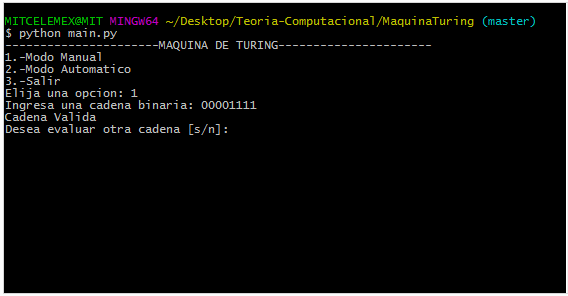
\includegraphics[width=\textwidth, height=7cm]{ModoManualTuring.png}
\label{fig:manual_webay}
\caption{La cadena a evaluar ser\'a 00001111}
\end{figure}

\begin{figure}[H]
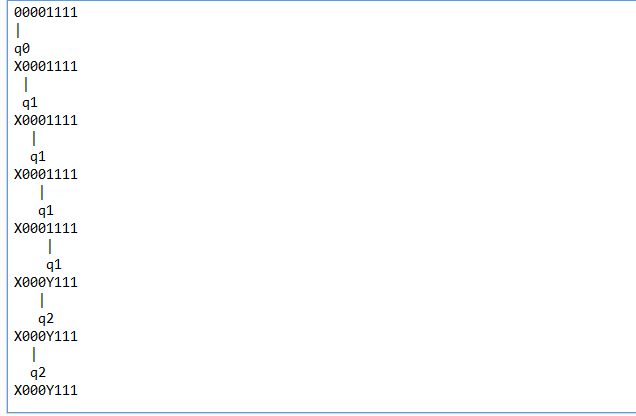
\includegraphics[width=\textwidth, height=7cm]{ArchivoTuring.png}
\label{fig:manualtexto_alfabeto}
\caption{Fragmento de la evaluaci\'on de la Maquina de Turing}
\end{figure}

Para el modo autom\'atico:\\
\begin{figure}[H]
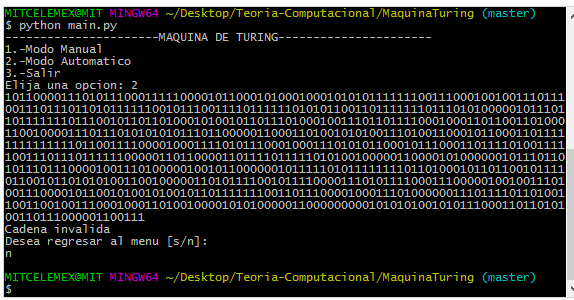
\includegraphics[width=\textwidth, height=7cm]{ModoAutomaticoTuring.png}
\label{fig:auto_alfabeto}
\caption{Tama\~no y cadena generado autom\'aticamente}
\end{figure}

\begin{figure}[H]
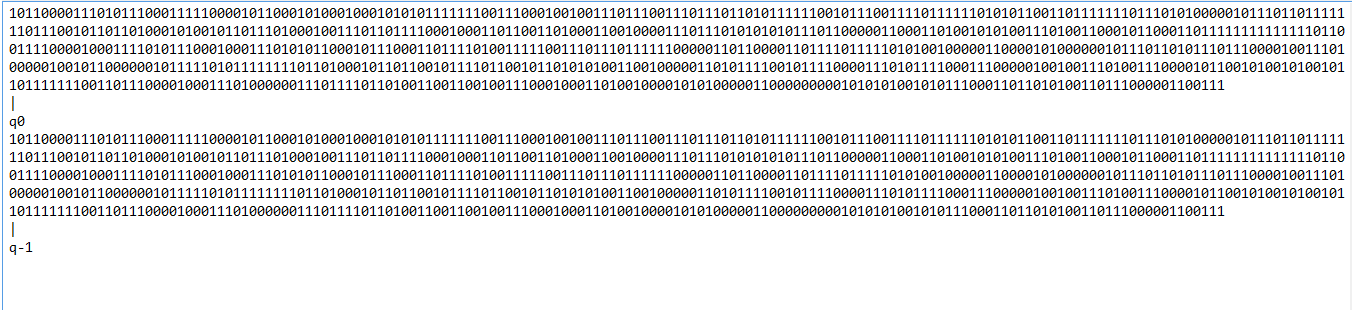
\includegraphics[width=\textwidth, height=7cm]{ArchivoHistoriaTuring.png}
\label{fig:autotexto_alfabeto}
\caption{Historia de la evaluaci\'on del modo autom\'atico}
\end{figure}

\begin{figure}[H]
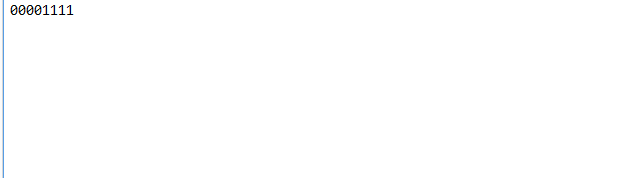
\includegraphics[width=\textwidth, height=7cm]{ValidasTuring.png}
\label{fig:manualtexto_alfabeto}
\caption{Cadenas validas aceptadas}
\end{figure}

\newpage